\chapter{Congestion and Flow Control}
\textbf{Intro}
\\\\
Rate limiting is not enough Of course and Congestion control mechanism for better servicing will be necessary. imagine many clients with huge amount of traffic use the same circuit, the consequence will be that the circuit might become saturated by a time. another scenario might be that an attacker sends a huge amount of data that do not read it at the end. so here some congestion control and flow control mechanism is needed, we will describe the Tors approach for the problem.
\\\\
\section{Tors Approach}
Tor will use two methods for solution that the second uses a modified version of first solution. the first solution will discuss about congestion control for circuits and then the second solution will discuss on multiple streams that are going through that circuit.
\\
\subsection{Circuit-level throttling}
To control a circuit’s bandwidth
usage, each OR keeps track of two windows. (See Fig \ref{fig:CongestionTor}) The packaging
window tracks how many relay data cells the OR is allowed to
package (from incoming TCP streams) for transmission back
to the OP, and the delivery window tracks how many relay
data cells it is willing to deliver to TCP streams outside the
network. Each window is initialized (say, to 1000 data cells).\\
\begin{figure}[!h]
\centering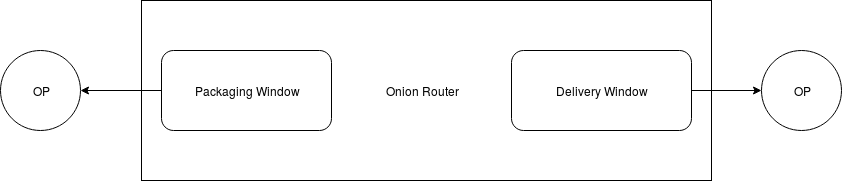
\includegraphics[scale=0.4]{CongestionTor}
\caption{The delivery and packaging window in a OR/OP}
\label{fig:CongestionTor} % Unique label used for referencing the figure in-text
\end{figure}
\\
When a data cell is packaged or delivered, the appropriate
window is decremented. When an OR has received enough
data cells (currently 100, see dir-spec.txt), it sends a relay sendme cell towards
the OP, with streamID zero. When an OR receives a relay
sendme cell with streamID zero (The body SHOULD be ignored)
, it increments its packaging window. Either of these cells increments the corresponding
window by 100. If the packaging window reaches 0, the OR
stops reading from TCP connections for all streams on the
corresponding circuit, and sends no more relay data cells until
receiving a relay sendme cell. You can see the sample scenario in Fig \ref{fig:CongestionTor2} .
\\
The OP behaves identically, except that it must track a
packaging window and a delivery window for every OR in
the circuit. If a packaging window reaches 0, it stops reading
from streams destined for that OR.
\\
An OR or OP sends cells to increment its delivery window when the
corresponding window value falls under some threshold (900).
\\
\begin{figure}[!h]
\centering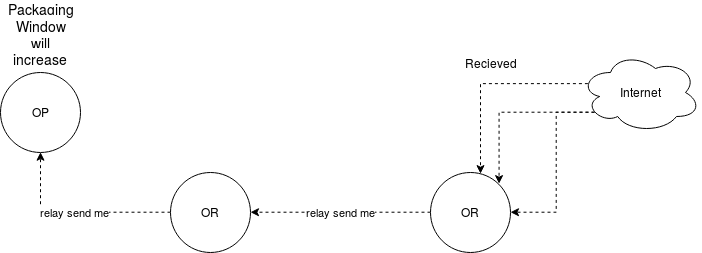
\includegraphics[scale=0.4]{CongestionTor2}
\caption{Circuit-level Congestion Control Scenario}
\label{fig:CongestionTor2} % Unique label used for referencing the figure in-text
\end{figure}
\\
\subsection{Stream-level throttling}
Stream-level Congestion Control is the same, ORs
and OPs use relay sendme cells to implement end-to-end flow
control for individual streams across circuits. \\
Each stream
begins with a packaging window (currently 500 cells), and
increments the window by a fixed value (50) upon receiving a relay sendme cell. \\
 Rather than always returning a relay
sendme cell as soon as enough cells have arrived, the stream level congestion control also has to check whether data has
been successfully flushed onto the TCP stream; it sends the
relay sendme cell only when the number of bytes pending to
be flushed is under some threshold (currently 10 cells worth).\\
for further information please refer to Section 8 of TorDesign. \cite{tor_paper}\\
Stream-level RELAY\_SENDME cells are distinguished by having nonzero
StreamID. They are still empty; the body still SHOULD be ignored.\\